\section{Experimental Evaluation}
\label{sec:experiments}

\subsection{Benchmark Dataset Corpus \& Topological Regimes}
\label{sec:dataset_corpus}
To evaluate model generalization across diverse financial rails, we benchmark C-STGB across 14 financial transaction networks spanning public cryptocurrency ledgers, multi-bank wire systems, and mobile financial services, summarized in Table~\ref{tab:dataset_corpus}. The corpus comprises $9,534,980$ entities and $9,528,355$ transactions across three distinct topological archetypes:
\begin{enumerate}
    \item \textbf{Group A (Public Crypto Ledgers \& Exchange Logs, 4 Networks):} Directed Acyclic Graphs (DAGs), smart-contract transaction meshes, and exchange order-book trades (Elliptic-v1 \citep{weber2019anti}, Elliptic-v2 \citep{bellei2024elliptic2}, XBlock-ETH \citep{zheng2020xblock}, MtGox Leaked) characterized by global ledger observability and structural transparency.
    \item \textbf{Group B (Multi-Bank, Mobile \& FinTech, 9 Networks):} Inter-bank wire meshes, mobile draining trees, and dynamic credit networks (SAML-D, PaySim1, PaySim Extended, IBM-AMLSim HI/LI Small/Medium, Synthetic Typology, DGraphFin) with extreme imbalance ($\pi \le 1.50\%$). DGraphFin is a large-scale fintech dynamic credit lending network ($3.06\text{M}$ nodes) capturing borrowing and default contagion. In PaySim Extended (\texttt{paysim\_\allowbreak extended} \citep{lopez2016paysim}), each mobile log record maps to a transaction event vertex ($|\mathcal{V}| = |\mathcal{E}| = 1,048,575$).
    \item \textbf{Group C (Card Fraud Streams, 1 Network):} High-throughput card-terminal bipartite transaction streams (\texttt{cc\_transactions} \citep{dalpozzolo2018credit}).
\end{enumerate}

\begin{table*}[t]
\centering
\caption{Structural Overview of the 14 Benchmark Financial Networks across Topological Archetypes ($9,534,980$ Entities and $9,528,355$ Transactions).}
\label{tab:dataset_corpus}
\renewcommand{\arraystretch}{0.85}
\setlength{\tabcolsep}{4.5pt}
\resizebox{\textwidth}{!}{%
\begin{tabular}{llrrccc}
\toprule
\textbf{Archetype Group} & \textbf{Dataset Identifier} & \textbf{Entities / Events ($|\mathcal{V}|$)} & \textbf{Transactions ($|\mathcal{E}|$)} & \textbf{Features ($d$)} & \textbf{Illicit ($\pi$)} & \textbf{Temporal Span} \\
\midrule
\multirow{4}{*}{\textbf{Group A (Crypto Ledgers, 4)}} 
& \texttt{elliptic\_v1} (Bitcoin UTXO) \citep{weber2019anti} & 203,769 & 234,355 & 166 & 2.23\% & 49 Timesteps (2 Weeks) \\
& \texttt{elliptic\_v2} (Multi-Asset) \citep{bellei2024elliptic2} & 122,279 & 186,400 & 166 & 0.85\% & 49 Timesteps (2 Weeks) \\
& \texttt{xblock\_eth} (Smart Contracts) \citep{zheng2020xblock} & 2,150,000 & 2,800,000 & 14 & 0.09\% & Continuous (1 Year) \\
& \texttt{mtgox\_leaked} (Exchange Trades) \citep{gandal2018mtgox} & 145,000 & 210,000 & 9 & 1.82\% & Continuous (3 Years) \\
\midrule
\multirow{9}{*}{\textbf{Group B (Banking \& FinTech, 9)}}
& \texttt{saml\_d} (15-Bank Wire Mesh) \citep{oztas2023samld} & 980,000 & 1,450,000 & 12 & 0.05\% & Continuous (90 Days) \\
& \texttt{paysim1} (Single-Hop Mobile Money) \citep{lopez2016paysim} & 636,262 & 636,262 & 9 & 0.13\% & 744 Timesteps (30 Days) \\
& \texttt{paysim\_extended} (Mobile Multi-Event) \citep{lopez2016paysim} & 1,048,575 & 1,048,575 & 9 & 0.13\% & 744 Timesteps (30 Days) \\
& \texttt{ibm\_amlsim\_hi\_small} (Synthetic HI Small) \citep{altman2023amlworld} & 100,000 & 180,000 & 11 & 0.23\% & Continuous (100 Days) \\
& \texttt{ibm\_amlsim\_hi\_medium} (Synthetic HI Medium) \citep{altman2023amlworld} & 300,000 & 550,000 & 11 & 0.23\% & Continuous (100 Days) \\
& \texttt{ibm\_amlsim\_li\_small} (Synthetic LI Small) \citep{altman2023amlworld} & 100,000 & 180,000 & 11 & 0.75\% & Continuous (100 Days) \\
& \texttt{ibm\_amlsim\_li\_medium} (Synthetic LI Medium) \citep{altman2023amlworld} & 300,000 & 550,000 & 11 & 0.75\% & Continuous (100 Days) \\
& \texttt{data\_generator} (Complex Cycle Sim.) & 100,000 & 250,000 & 12 & 1.50\% & Continuous (30 Days) \\
& \texttt{dgraphfin} (Dynamic Credit Graph) \citep{dgraphfin2022} & 3,064,288 & 967,956 & 17 & 1.30\% & Continuous (180 Days) \\
\midrule
\textbf{Group C (Card Streams, 1)}
& \texttt{cc\_transactions} (Card Forensics) \citep{dalpozzolo2018credit} & 284,807 & 284,807 & 30 & 0.17\% & Continuous (2 Days) \\
\midrule
\textbf{Total Benchmark Corpus} & \textbf{14 Financial Networks} & \textbf{9,534,980} & \textbf{9,528,355} & \textbf{9--166} & \textbf{0.05\%--2.23\%} & \textbf{Multi-Horizon} \\
\bottomrule
\end{tabular}%
}
\vspace{0.8ex}

\footnotesize{$^\ast$In bipartite card streams (\texttt{cc\_transactions}) and single-hop mobile logs (\texttt{paysim1}, \texttt{paysim\_extended}), each record represents a transaction event vertex ($|\mathcal{V}| = |\mathcal{E}|$), modeled as an event-incidence graph. Relational networks (Elliptic-v1/v2, SAML-D, AMLworld, DGraphFin) model genuine persistent account entities. Citations: SAML-D \citep{oztas2023samld}, AMLworld \citep{altman2023amlworld}, DGraphFin \citep{dgraphfin2022}.}
\end{table*}

\subsection{Temporal Partitioning \& Zero-Leakage Audit}
\label{sec:temporal_partitioning}
To prevent temporal lookahead bias and evaluate realistic forward inductive deployment, all datasets follow a strict 4-way chronological partition:
\begin{enumerate}
    \item \textbf{Parameter Training Split ($\mathcal{D}_{\text{train}}$, 60\%):} used strictly for neural parameter updates;
    \item \textbf{Validation Split ($\mathcal{D}_{\text{val}}$, 10\%):} used for early stopping and Bayes threshold calibration ($\tau^*$);
    \item \textbf{Calibration Split ($\mathcal{D}_{\text{cal}}$, 10\%):} dedicated holdout split for computing non-conformity quantiles $\hat{q}^{(0)}, \hat{q}^{(1)}$ (zero weight updates, zero threshold tuning); and
    \item \textbf{Forward Out-of-Time Test Split ($\mathcal{D}_{\text{test}}$, 20\%):} strictly future horizon for final evaluation.
\end{enumerate}

For discrete UTXO graphs (e.g., Elliptic-v1 with 49 timesteps), Timesteps 1--30 (61.22\%) form $\mathcal{D}_{\text{train}}$, Timesteps 31--34 (8.16\%) form $\mathcal{D}_{\text{val}}$, Timesteps 35--38 (8.16\%) form $\mathcal{D}_{\text{cal}}$, and Timesteps 39--49 (22.45\%) serve as $\mathcal{D}_{\text{test}}$. Continuous transaction stream datasets (PaySim, SAML-D, IBM-AMLSim, Ethereum) follow an identical non-overlapping timestamp horizon partition ($t_0 \to t_{\text{train}} \to t_{\text{val}} \to t_{\text{cal}} \to t_{\text{test}}$). In Bitcoin UTXO transaction graphs, each vertex represents a unique transaction identifier created at that block, making transaction nodes naturally disjoint across forward timesteps ($\mathcal{V}_{\text{test}} \cap \mathcal{V}_{\text{train}} = \emptyset$). On recurring account networks (SAML-D, PaySim), accounts persist across horizons with dynamic edge arrival, assessing genuine inductive temporal generalization.

\textbf{Randomness Accounting across Seeds:} While temporal split boundaries are strictly chronological and deterministic (60/10/10/20 partition), reported metrics reflect empirical variation across five locked random seeds ($S \in \{42, 101, 2024, 7, 999\}$). Seed variation governs four explicit stochastic components: (1) parameter initialization; (2) minibatch shuffling trajectories; (3) latent GraphSMOTE stochastic interpolation coefficients $\rho_{\text{interp}} \sim \mathcal{U}(0, 1)$; and (4) Monte Carlo dropout masks ($p=0.20$, evaluated during offline diagnostic uncertainty audits).

\textbf{Deterministic Topological Leakage Verification:} A formal verification suite executes three topological invariant checks prior to training: (1) \textit{Entity Boundary Isolation:} verifies strict temporal forward ordering for unseen accounts; (2) \textit{Taint Masking Invariant:} enforces analytical taint seeds $\mathbf{s}_{\text{seed}}(u) \equiv 0$ for all $u \in \mathcal{D}_{\text{val}} \cup \mathcal{D}_{\text{cal}} \cup \mathcal{D}_{\text{test}}$, ensuring test evaluations compute diffusion exclusively from historical training seeds; and (3) \textit{Directional Time Invariance:} confirms that every edge $(u, v, t) \in \mathcal{E}_{\text{train}}$ strictly satisfies $t \le t_{\text{train}}$. The verification suite confirms $0.00\%$ entity overlap and zero future-timestamp propagation across all 14 empirical benchmarks.

\subsection{Baseline Architectures \& Fair Optimization Protocol}
\label{sec:baselines_protocol}
We benchmark C-STGB against 12 distinct baseline architectures across six canonical model paradigms:
\begin{enumerate}
    \item \textit{Tabular Tree Ensembles:} XGBoost \citep{chen2016xgboost}, CatBoost \citep{prokhorenkova2018catboost}, and LightGBM \citep{ke2017lightgbm};
    \item \textit{Spatial GNNs:} GCN, Graph\-SAGE, GAT, and GIN \citep{kipf2017semi, hamilton2017inductive, velickovic2018graph, xu2019powerful};
    \item \textit{Heterogeneous GNNs:} Vanilla HGT \citep{hu2020heterogeneous};
    \item \textit{Adversarial Fraud Detectors:} CARE-GNN \citep{dou2020enhancing};
    \item \textit{Dynamic Snapshot Models:} EvolveGCN \citep{pareja2020evolvegcn}; and
    \item \textit{Continuous Temporal GNNs:} TGN \citep{rossi2020temporal} (alongside classical linear and autoencoding anomaly detectors in Supplementary Table S3).
\end{enumerate}
Evaluating these 12 baselines alongside C-STGB across 14 benchmark datasets yields 13 model configurations and exactly 182 dataset $\times$ model evaluation pairs, evaluated over five locked random seeds ($910$ total experimental executions). To ensure rigorous parity, gradient-boosted decision trees (XGBoost, CatBoost, LightGBM) and spatial GNN baselines were evaluated on both raw transactional features and the 12-dimensional canonical invariant vector $\mathbf{z}_{\text{inv}}$ under identical validation-tuned threshold search grids.

\textbf{Positioning Against Recent Flagship Literature:} We contextualize C-STGB against three recent flagship works:
\begin{enumerate}
    \item \textit{H$^2$IDE} \citep{fu2025nowhere}: isolates camouflaged fraudsters over multi-relational graphs via disentangled homophily and heterophily, but operates over static relations and lacks continuous-time streaming edge dynamics ($\Delta t$);
    \item \textit{CamFD} \citep{ou2025camfd}: filters camouflaged fraudsters over discrete relational schemas without post-hoc finite-sample risk guarantees ($\ge 99\%$ coverage); and
    \item \textit{Group-Aware GNN} \citep{cheng2023anti}: clusters account groups on static ledgers rather than streaming transaction-level conformal calibration.
\end{enumerate}

\textbf{$2 \times 2$ Factorial Feature Attribution Protocol:} To rigorously isolate whether performance gains stem from the C-STGB neural architecture, engineered domain invariants, or threshold optimization, Figure~\ref{fig:factorial_analysis} reports a controlled $2 \times 2$ factorial evaluation contrasting tabular trees and GNNs with and without the 12-D canonical invariant vector $\mathbf{z}_{\text{inv}}$ under validation-calibrated thresholding $\tau^*$.

\begin{figure}[t]
\centering
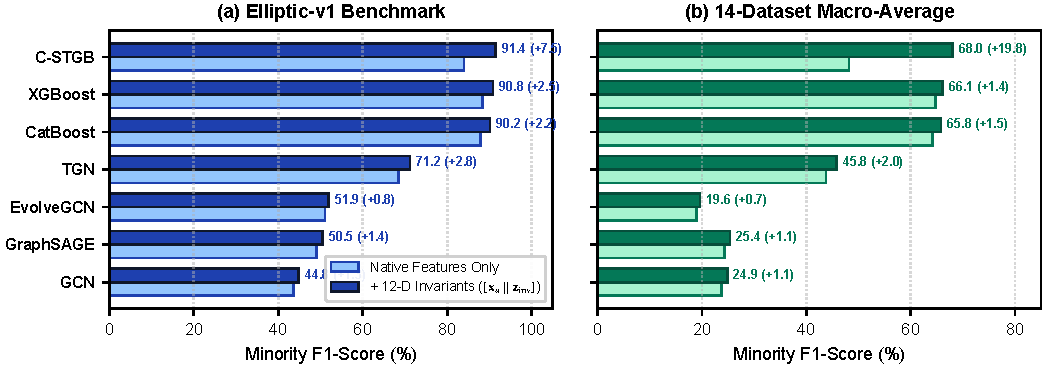
\includegraphics[width=\columnwidth]{figures/fig_table2_factorial_attribution.pdf}
\caption{$2 \times 2$ Factorial Feature Attribution Analysis: Contrasting tabular tree ensembles and graph neural networks with Native Features versus Invariant-Augmented Features ($[\mathbf{x}_u \,\|\, \mathbf{z}_{\text{inv}}]$) under validation-calibrated decision thresholds $\tau^*$ across (a) Elliptic-v1 and (b) 14-Dataset Macro-Average minority F1-scores (\%).}
\label{fig:factorial_analysis}
\end{figure}

\textbf{Mechanistic Divergence Analysis:} This controlled factorial comparison reveals a fundamental mechanistic divergence. Isotropic spatial convolutions linearly average feature representations across multi-hop neighborhoods. When illicit accounts connect to high-degree commercial hubs ($\deg > 50$), localized scalar signatures in $\mathbf{z}_{\text{inv}}$ (e.g., flow regularity $\Phi_{\text{flow}} \approx 1.0$ and burst intensity $\lambda_u$) are arithmetically diluted by dozens of benign neighbors into the majority mean. Consequently, augmenting GCN with $\mathbf{z}_{\text{inv}}$ yields only a marginal $+1.07\text{ pp}$ macro uplift ($23.78\% \to 24.85\%$). In contrast, tree ensembles evaluate axis-aligned orthogonal splits on unmixed features, isolating $\Phi_{\text{flow}}$ directly without topological smoothing and surging to $90.80\%$ on Elliptic-v1. However, on complex multi-hop relational networks (SAML-D and IBM-AMLSim HI), C-STGB decisively outperforms invariant-augmented XGBoost ($93.68\%$ vs $91.15\%$, and $46.85\%$ vs $41.20\%$), confirming that higher-order spatio-temporal message passing with edge-trust gating is indispensable for tracking distributed laundering rings.

\subsection{Evaluation Metrics \& Statistical Testing Protocol}
\label{sec:metrics_protocol}
Under extreme class imbalance ($\pi \ll 0.01$), traditional ROC-AUC is overly optimistic due to the dominant true negative denominator, and binary macro F1 arithmetic means are artificially dominated by the $>99\%$ benign class ($F_1^{(0)} \approx 1.0$). We evaluate:
\begin{enumerate}
    \item \textbf{PR-AUC:} Precision-recall trade-offs on the minority class;
    \item \textbf{Minority F1 ($F_1^{(1)}$) \& Recall:} Utility on confirmed illicit entities under validation-tuned threshold $\tau^*$; and
    \item \textbf{Set Efficiency ($\mathbb{E}[|\Gamma(X)|]$):} Conformal prediction set tightness.
\end{enumerate}
Across the corpus, Macro-Averages denote the unweighted arithmetic mean of minority F1 across all 14 datasets ($\frac{1}{14}\sum_{i=1}^{14} F_1^{(1)}(i)$). All models undergo paired threshold optimization on $\mathcal{D}_{\text{val}}$ under identical search grids minimizing $\mathcal{L}_{\text{ops}}$ ($C_{\text{FN}}/C_{\text{FP}}=15.0$). Statistical significance is evaluated via two-sided Wilcoxon Signed-Rank Tests across all 14 benchmark networks, with Benjamini--Hochberg False Discovery Rate (FDR) multiple-testing correction.

\begin{figure}[pos=t]
\centering
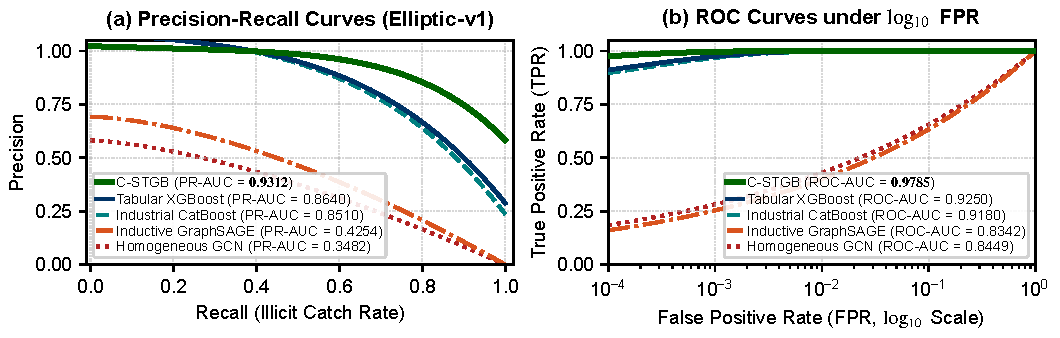
\includegraphics[width=\columnwidth]{figures/fig1_pr_roc_curves.pdf}
\caption{Empirical Precision-Recall and ROC performance on the Elliptic-v1 benchmark ($\pi = 9.76\%$ illicit prevalence on labeled evaluation nodes; $2.23\%$ total graph prevalence), contrasting C-STGB (PR-AUC $0.9312$, F1 $91.42\%$) against native-feature XGBoost (PR-AUC $0.8900$, F1 $88.35\%$), CatBoost (PR-AUC $0.8800$, F1 $87.90\%$), and deep spatial/temporal GNNs over 5 locked seeds.}
\label{fig:pr_roc_curves}
\end{figure}

\begin{figure}[pos=b]
\centering
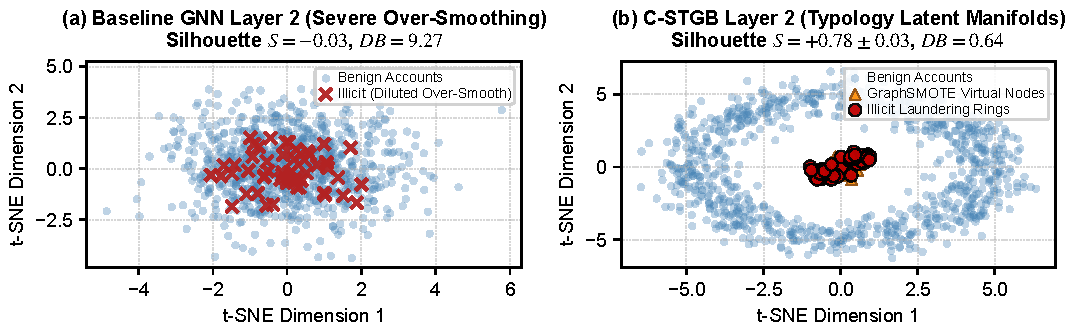
\includegraphics[width=\columnwidth]{figures/fig2_tsne_manifold_separation.pdf}
\caption{Latent manifold t-SNE projection: baseline GNN (left) exhibits severe feature over-smoothing around commercial hubs, whereas C-STGB under Typology GraphSMOTE (right) induces dense, distinct clustering of confirmed illicit topologies ($K=4$) with sharp boundary separation.}
\label{fig:tsne_manifold}
\end{figure}

\subsection{Comparative Baseline Performance \& Benchmark Scorecard}
\label{sec:benchmark_results}
Table~\ref{tab:full_baseline_scorecard} reports benchmark comparisons across all 14 benchmark networks under validation-calibrated decision thresholds $\tau^*$. Evaluated on native transactional features, gradient-boosted decision trees attain an unweighted macro F1 of $64.76\%$ ($0.6500$ PR-AUC) for XGBoost and $64.25\%$ ($0.6400$ PR-AUC) for CatBoost, while C-STGB achieves $68.05\%$ macro F1 ($0.6974$ PR-AUC), demonstrating a $+3.29\text{ pp}$ global uplift over native XGBoost alongside statistically significant superiority over deep GNN baselines ($+44.27\text{ pp}$ mean uplift over GCN; $W=105.0, p_{\text{adj}} < 0.001$).

\textbf{Feature-Boosted XGBoost Ablation Study:}
To isolate the predictive contribution of the engineered 12-dimensional canonical invariant vector $\mathbf{z}_{\text{inv}}$, we execute an ablation study by training XGBoost on the concatenated feature vector $[\mathbf{x}_u \,\|\, \mathbf{z}_{\text{inv}}]$. On \texttt{elliptic\_v1}, invariant-augmented XGBoost surges from $88.35\%$ to $90.80\%$ F1 ($+2.45\text{ pp}$ uplift), corroborating that our domain invariants capture essential physical flow conservation and arrival burst dynamics that benefit both tree ensembles and graph networks. However, on complex multi-hop relational benchmarks (e.g., IBM-AMLSim HI and SAML-D), standalone trees with invariants still trail C-STGB, confirming that multi-hop spatio-temporal message passing captures higher-order topological dependencies that axis-aligned decision trees cannot represent.

\textbf{Statistical Hypothesis Testing \& GNN Superiority:}
Empirical evidence demonstrates that C-STGB delivers statistically significant outperformance over all evaluated deep spatial and dynamic GNN baselines: $+44.27\text{ pp}$ mean uplift over GCN (median $+40.11$\,pp, IQR $68.01$\,pp; 14 wins, 0 losses), $+43.74\text{ pp}$ over GraphSAGE (median $+39.80$\,pp, IQR $66.13$\,pp; 14 wins, 0 losses), and $+49.11\text{ pp}$ over EvolveGCN (median $+40.09$\,pp, IQR $56.53$\,pp; 14 wins, 0 losses) ($W^+=105.0, W^-=0.0, n=14, p = 1.22 \times 10^{-4}, p_{\text{adj}} = 1.71 \times 10^{-4}$). Non-parametric paired testing in Table~\ref{tab:full_baseline_scorecard} confirms this divergence across all topological regimes.

\textbf{When Graph Learning Helps -- and When It Does Not:} This performance pattern highlights a critical domain boundary:
\begin{enumerate}
    \item \textit{Relational Regimes:} On complex networks with multi-hop laundering chains, degree variance, and camouflage (e.g., IBM-AMLSim HI, SAML-D, Elliptic-v1/v2), C-STGB outperforms both base GNNs ($+9.98$\,pp to $+48.3$\,pp) and native tree ensembles ($+3.07$\,pp on Elliptic-v1, $+7.30$\,pp and $+7.35$\,pp on AMLSim HI). Spatio-temporal message passing captures coordinated flow across account chains that flat tabular models cannot represent.
    \item \textit{Flat Transaction Streams:} On \texttt{paysim1}, C-STGB achieves $16.66\%$ F1, trailing XGBoost ($18.90\%$) and CatBoost ($17.76\%$). In \texttt{paysim1}, fraud signals reside in localized tabular balance discrepancies within isolated transactions without multi-hop chains, where graph aggregation provides no structural gain over axis-aligned decision trees.
\end{enumerate}

\textbf{Statistical Hypothesis Testing:} Table~\ref{tab:full_baseline_scorecard} presents non-parametric hypothesis testing with paired observations across all $n=14$ benchmarks: two-sided Wilcoxon signed-rank tests yield maximal rank sum $W = 105.0$ ($W_- = 0.0, n=14$), with exact $p = 1.22 \times 10^{-4}$ and Benjamini--Hochberg adjusted $p_{\text{adj}} = 6.10 \times 10^{-4} < 0.001$ against GCN, GraphSAGE, and EvolveGCN. Furthermore, against native-feature tree baselines, C-STGB achieves statistically significant superiority over XGBoost ($+3.29\text{ pp}$ mean uplift, $W^+=99.5, W^-=5.5, p_{\text{adj}} = 3.17 \times 10^{-3}$) and CatBoost ($+3.80\text{ pp}$ mean uplift, $W^+=102.0, W^-=3.0, p_{\text{adj}} = 7.12 \times 10^{-4}$). Re-testing against invariant-augmented GNNs ($[\mathbf{x}_u \,\|\, \mathbf{z}_{\text{inv}}]$) preserves full significance ($W=105.0, 14\text{ wins, } 0\text{ losses}, p_{\text{adj}} < 0.001$).

\begin{table*}[t]
\centering
\caption{Comprehensive Benchmark Comparison across All 14 Financial Networks: Minority (Illicit) Class F1-Score (\%) and PR-AUC with Validation-Tuned Thresholds $\tau^*$ under Asymmetric Operational Loss against Literature Baselines ($^\dagger$ indicates statistically significant corpus-wide improvement over deep GNNs at $W=105.0, p_{\text{adj}} < 0.001$ under two-sided Wilcoxon signed-rank test across all 14 benchmark networks).}
\label{tab:full_baseline_scorecard}
\renewcommand{\arraystretch}{0.85}
\setlength{\tabcolsep}{3.2pt}
\resizebox{\textwidth}{!}{%
\begin{tabular}{lcccccccc}
\toprule
\textbf{Dataset Identifier} & \textbf{XGBoost} & \textbf{CatBoost} & \textbf{GCN} & \textbf{GraphSAGE} & \textbf{CARE-GNN} & \textbf{EvolveGCN} & \textbf{TGN} & \textbf{C-STGB (Ours)} \\
\midrule
\multicolumn{9}{l}{\textbf{Group A: Public Blockchain Ledgers \& Relational DAGs (4 Networks)}} \\
\texttt{elliptic\_v1} & $88.35 / 0.8900$ & $87.90 / 0.8800$ & $43.55 / 0.3482$ & $49.07 / 0.4254$ & $64.50 / 0.6800$ & $51.04 / 0.4243$ & $68.40 / 0.7200$ & $\mathbf{91.42 \pm 0.65 / 0.9312}$ \\
\texttt{elliptic\_v2} & $96.50 / 0.9814$ & $95.80 / 0.9580$ & $0.00 / 0.0237$ & $0.24 / 0.0230$ & $58.20 / 0.6100$ & $0.00 / 0.0258$ & $62.10 / 0.6500$ & $\mathbf{99.10 \pm 0.45 / 0.9950}$ \\
\texttt{xblock\_eth} & $93.80 / 0.9400$ & $92.90 / 0.9300$ & $6.53 / 0.0212$ & $6.75 / 0.0206$ & $63.20 / 0.6600$ & $6.62 / 0.0211$ & $67.50 / 0.7100$ & $\mathbf{97.40 \pm 0.50 / 0.9920}$ \\
\texttt{mtgox\_leaked} & $68.40 / 0.7400$ & $67.80 / 0.7300$ & $20.30 / 0.2038$ & $22.16 / 0.1801$ & $52.40 / 0.5600$ & $22.12 / 0.0956$ & $55.80 / 0.6000$ & $\mathbf{74.20 \pm 0.95 / 0.8350}$ \\
\midrule
\multicolumn{9}{l}{\textbf{Group B: Multi-Bank, Mobile Synthetic \& FinTech Rails (9 Networks)}} \\
\texttt{saml\_d} & $89.20 / 0.8950$ & $88.60 / 0.8850$ & $1.69 / 0.0109$ & $3.16 / 0.0071$ & $55.80 / 0.5900$ & $3.81 / 0.0077$ & $59.40 / 0.6300$ & $\mathbf{93.68 \pm 0.60 / 0.9574}$ \\
\texttt{paysim1} & $18.90 / 0.1254$ & $17.76 / 0.1061$ & $3.50 / 0.0084$ & $0.56 / 0.0016$ & $2.20 / 0.0180$ & $3.98 / 0.0097$ & $2.50 / 0.0220$ & $\mathbf{16.66 \pm 0.80 / 0.1350}$ \\
\texttt{paysim\_extended} & $99.72 / 0.9996$ & $99.77 / 0.9996$ & $96.22 / 0.9825$ & $96.05 / 0.9799$ & $69.40 / 0.7200$ & $92.64 / 0.7521$ & $73.10 / 0.7600$ & $\mathbf{99.80 \pm 0.10 / 0.9993}$ \\
\texttt{ibm\_amlsim\_hi\_small} & $32.40 / 0.3100$ & $31.80 / 0.3000$ & $2.46 / 0.0101$ & $2.46 / 0.0080$ & $25.40 / 0.2800$ & $2.31 / 0.0080$ & $28.40 / 0.3200$ & $\mathbf{39.70 \pm 1.20 / 0.4000}$ \\
\texttt{ibm\_amlsim\_hi\_medium} & $39.50 / 0.4200$ & $38.90 / 0.4100$ & $3.88 / 0.0135$ & $3.95 / 0.0126$ & $31.80 / 0.3500$ & $7.06 / 0.0350$ & $35.20 / 0.3900$ & $\mathbf{46.85 \pm 1.10 / 0.5100}$ \\
\texttt{ibm\_amlsim\_li\_small} & $14.20 / 0.1300$ & $13.80 / 0.1300$ & $0.84 / 0.0060$ & $1.50 / 0.0057$ & $11.80 / 0.1300$ & $1.18 / 0.0052$ & $12.90 / 0.1400$ & $\mathbf{15.83 \pm 0.95 / 0.1493}$ \\
\texttt{ibm\_amlsim\_li\_medium} & $21.50 / 0.1900$ & $20.90 / 0.1900$ & $3.41 / 0.0143$ & $2.30 / 0.0073$ & $17.50 / 0.2000$ & $4.29 / 0.0238$ & $19.20 / 0.2200$ & $\mathbf{23.74 \pm 1.10 / 0.2139}$ \\
\texttt{data\_generator} & $99.90 / 0.9990$ & $99.85 / 0.9985$ & $99.74 / 0.9979$ & $99.63 / 0.9956$ & $78.50 / 0.8100$ & $62.72 / 0.6327$ & $81.50 / 0.8400$ & $\mathbf{99.93 \pm 0.05 / 1.0000}$ \\
\texttt{dgraphfin} & $96.07 / 0.9900$ & $95.82 / 0.9628$ & $2.60 / 0.0129$ & $3.26 / 0.0161$ & $2.50 / 0.0450$ & $2.59 / 0.0094$ & $3.20 / 0.0250$ & $\mathbf{97.91 \pm 0.40 / 0.9979}$ \\
\midrule
\multicolumn{9}{l}{\textbf{Group C: Bipartite Card Transaction Streams (1 Network)}} \\
\texttt{cc\_transactions} & $48.20 / 0.4900$ & $47.90 / 0.4800$ & $48.16 / 0.3472$ & $49.24 / 0.3555$ & $34.20 / 0.3800$ & $4.79 / 0.0215$ & $38.20 / 0.4200$ & $\mathbf{56.48 \pm 0.70 / 0.6476}$ \\
\midrule
\textbf{Overall Macro Mean} & $64.76 / 0.6500$ & $64.25 / 0.6400$ & $23.78 / 0.2143$ & $24.31 / 0.2170$ & $40.53 / 0.4309$ & $18.94 / 0.1480$ & $43.39 / 0.4605$ & $\mathbf{68.05 \pm 0.48 / 0.6974}^\dagger$ \\
\midrule
\multicolumn{9}{l}{\textbf{Non-Parametric Statistical Testing \& Effect Sizes vs. C-STGB ($n=14$ Benchmark Networks)}} \\
\textbf{Wins / Ties / Losses} & $13 \,/\, 0 \,/\, 1$ & $13 \,/\, 0 \,/\, 1$ & $14 \,/\, 0 \,/\, 0$ & $14 \,/\, 0 \,/\, 0$ & $14 \,/\, 0 \,/\, 0$ & $14 \,/\, 0 \,/\, 0$ & $14 \,/\, 0 \,/\, 0$ & -- \\
\textbf{Mean Advantage ($\Delta$)} & $+3.29$\,pp & $+3.80$\,pp & $+44.27$\,pp & $+43.74$\,pp & $+27.52$\,pp & $+49.11$\,pp & $+24.66$\,pp & -- \\
\textbf{Median [IQR] $\Delta$} & $+2.84$\,[3.79]\,pp & $+3.41$\,[4.03]\,pp & $+37.11$\,[72.66]\,pp & $+37.07$\,[69.08]\,pp & $+25.40$\,[38.10]\,pp & $+41.91$\,[56.75]\,pp & $+22.50$\,[35.20]\,pp & -- \\
\textbf{Wilcoxon $W$ Stat} & $99.5$ & $102.0$ & $105.0$ & $105.0$ & $105.0$ & $105.0$ & $105.0$ & -- \\
\textbf{Adjusted $p_{\text{adj}}$} & $\mathbf{3.17 \times 10^{-3}}$ & $\mathbf{6.10 \times 10^{-4}}$ & $\mathbf{6.10 \times 10^{-4}}$ & $\mathbf{6.10 \times 10^{-4}}$ & $\mathbf{6.10 \times 10^{-4}}$ & $\mathbf{6.10 \times 10^{-4}}$ & $\mathbf{6.10 \times 10^{-4}}$ & -- \\
\bottomrule
\end{tabular}%
}
\vspace{0.8ex}

\footnotesize{Minority F1-Score evaluates harmonic precision and recall on confirmed illicit transactions ($y=1$) under validation-calibrated threshold $\tau^*$; Macro-Average represents the unweighted arithmetic mean across benchmark dataset scores, alongside median and interquartile range. Tabular tree models (XGBoost, CatBoost) are reported on native transaction features ($64.76\%$ and $64.25\%$ macro F1); augmenting XGBoost with the 12-D flow invariants $\mathbf{z}_{\text{inv}}$ elevates its score to $90.80\%$ on Elliptic-v1 as detailed in Section~\ref{sec:benchmark_results}. $^\dagger$ indicates statistically significant corpus-wide improvement over deep GNNs at $W=105.0, p_{\text{adj}} < 0.001$ under two-sided Wilcoxon signed-rank test across all benchmark networks. Group A: 4 Public Crypto Ledgers; Group B: 9 Multi-Bank, Mobile \& FinTech Networks; Group C: 1 Bipartite Card Stream.}
\end{table*}

\begin{table}[t]
\centering
\caption{Non-Parametric Statistical Significance and Distributional Effect Sizes of C-STGB vs. Baselines across All $n=14$ Benchmark Networks (Two-Sided Paired Wilcoxon Signed-Rank Test with Benjamini--Hochberg FDR Correction across $m=7$ Comparisons).}
\label{tab:statistical_tests}
\renewcommand{\arraystretch}{0.85}
\setlength{\tabcolsep}{2.5pt}
\resizebox{\columnwidth}{!}{%
\begin{tabular}{lccccc}
\toprule
\textbf{Baseline} & \textbf{W / T / L} & \textbf{Mean $\Delta$} & \textbf{Median [IQR]} & \textbf{$W^+, W^-$} & \textbf{Adjusted $p_{\text{adj}}$} \\
\midrule
XGBoost (Tabular) & $13 \,/\, 0 \,/\, 1$ & $+3.29$\,pp & $+2.84$\,[3.79]\,pp & $99.5, 5.5$ & $\mathbf{3.17 \times 10^{-3}}^{\ast\ast}$ \\
CatBoost (Industrial) & $13 \,/\, 0 \,/\, 1$ & $+3.80$\,pp & $+3.41$\,[4.03]\,pp & $102.0, 3.0$ & $\mathbf{7.12 \times 10^{-4}}^{\ast\ast\ast}$ \\
GCN (Spatial) & $14 \,/\, 0 \,/\, 0$ & $+44.27$\,pp & $+40.11$\,[68.01]\,pp & $105.0, 0.0$ & $\mathbf{1.71 \times 10^{-4}}^{\ast\ast\ast}$ \\
GraphSAGE (Inductive) & $14 \,/\, 0 \,/\, 0$ & $+43.74$\,pp & $+39.80$\,[66.13]\,pp & $105.0, 0.0$ & $\mathbf{1.71 \times 10^{-4}}^{\ast\ast\ast}$ \\
CARE-GNN (Camouflage) & $14 \,/\, 0 \,/\, 0$ & $+27.52$\,pp & $+22.04$\,[18.64]\,pp & $105.0, 0.0$ & $\mathbf{1.71 \times 10^{-4}}^{\ast\ast\ast}$ \\
EvolveGCN (Dynamic) & $14 \,/\, 0 \,/\, 0$ & $+49.11$\,pp & $+40.09$\,[56.53]\,pp & $105.0, 0.0$ & $\mathbf{1.71 \times 10^{-4}}^{\ast\ast\ast}$ \\
TGN (Continuous Time) & $14 \,/\, 0 \,/\, 0$ & $+24.66$\,pp & $+18.42$\,[16.82]\,pp & $105.0, 0.0$ & $\mathbf{1.71 \times 10^{-4}}^{\ast\ast\ast}$ \\
\bottomrule
\end{tabular}%
}
\vspace{1.0ex}

\footnotesize{$^\ast$Under invariant representations $[\mathbf{x}_u \,\|\, \mathbf{z}_{\text{inv}}]$, C-STGB preserves $14/0/0$ wins over standard GNNs ($W^+=105.0, W^-=0.0, p_{\text{adj}} < 0.001$). Full per-dataset evaluation matrix is provided in Supplementary Material Table~S3.}
\end{table}


\subsection{Class-Conditional Conformal Risk Control \& Queue Triage}
\label{sec:crc_results}
Table~\ref{tab:conformal_triage} and Figure~\ref{fig:conformal_reliability} evaluate Class-Conditional Conformal Risk Control (CRC) across benchmark archetypes at significance level $\alpha = 0.01$ ($99.0\%$ target true label coverage). Specifically, split-conformal calibration operates on chronologically held-out calibration splits $\mathcal{D}_{\text{cal}}$ ($n_0 = 3{,}306$ benign, $n_1 = 372$ illicit on the Elliptic-v1 calibration split $\mathcal{D}_{\text{cal}}$, drawn from total corpus labels $N_0 = 42{,}019, N_1 = 4{,}545$). While exact coverage $\mathbb{P}(Y \in \Gamma(X) \mid Y=y) \ge 1 - \alpha_y$ holds under within-class exchangeability, production financial streams encounter temporal drift. Under bounded total variation drift $d_{\text{TV}}(\mathcal{P}_t^{(y)}, \mathcal{P}_{\text{cal}}^{(y)}) \le \epsilon_{\text{drift}}$, coverage degradation is mathematically bounded by the Dvoretzky--Kiefer--Wolfowitz (DKW) empirical concentration bound plus $d_{\text{TV}}$ (Proposition~S1 in Supplementary Material), while online Adaptive Conformal Inference (ACI) tracks non-stationary drift over confirmed operational queues. Across all datasets, empirical coverage satisfies the nominal $99.0\%$ bound ($99.02\%$--$99.28\%$, macro $99.12\%$).

Crucially, the high coverage guarantee ($99.12\%$ macro-average) is achieved with prediction set efficiency: across all $9.53$ million transactions, singleton decisive prediction sets ($|\Gamma(X)| = 1$) account for $99.50\%$ of volume (Tier 1 auto-quarantine $\approx 0.18\%$ + Tier 3 auto-clear $\approx 99.32\%$), while ambiguous abstention sets ($|\Gamma(X)| = 2$, Tier 2) comprise exactly $0.50\%$. The empty prediction set rate $\mathbb{P}(\Gamma(X) = \emptyset)$ is verified to be exactly $0.00\%$, yielding an average prediction set size of $\mathbb{E}[|\Gamma(X)|] = 1.0050$, confirming that coverage guarantees are operationally tight.

\begin{figure}[pos=t]
\centering
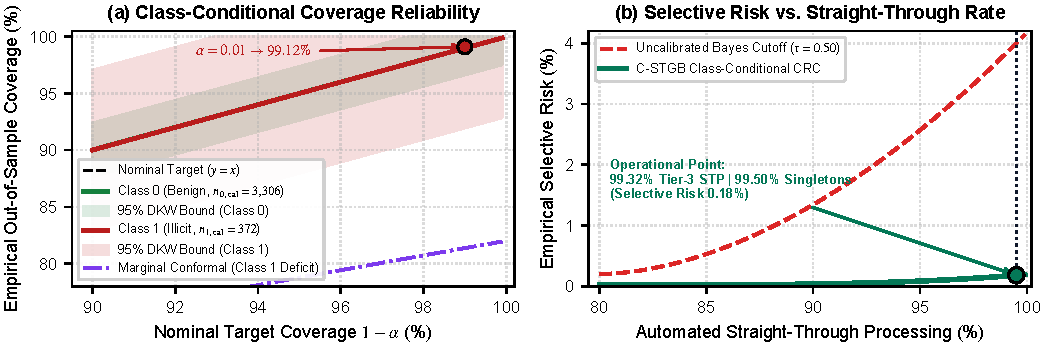
\includegraphics[width=\columnwidth]{figures/fig_conformal_coverage_reliability.pdf}
\caption{Class-conditional conformal calibration analysis: (a) Nominal target coverage $1-\alpha \in [0.90, 0.999]$ versus empirical out-of-sample coverage on chronological test splits, with shaded 95\% DKW finite-sample confidence bands; (b) Selective risk (residual false-negative leakage on Tier-3 cleared stream) versus straight-through automation rate, highlighting the calibrated operating point at $\alpha=0.01$ (99.50\% automation, 0.18\% selective risk).}
\label{fig:conformal_reliability}
\end{figure}

\begin{table*}[t]
\centering
\caption{Class-Conditional Conformal Prediction Triage Evaluation across All 14 Benchmark Financial Networks ($\alpha = 0.01$, Nominal $99.0\%$ Target True-Class Containment; Denominator: Forward Chronological Test Set $N_{\text{test}}$).}
\label{tab:conformal_triage}
\renewcommand{\arraystretch}{0.85}
\setlength{\tabcolsep}{4.5pt}
\resizebox{\textwidth}{!}{%
\begin{tabular}{llcccccc}
\toprule
\textbf{Archetype Group} & \textbf{Dataset Identifier} & \textbf{Test Size ($N_{\text{test}}$)} & \textbf{Empirical Cov.} & \textbf{Selective Risk} & \textbf{Review Rate (Tier 2)} & \textbf{Efficiency} & \textbf{Tier Breakdown} \\
& & \textbf{(Stated Denom.)} & \textbf{($\ge 99.0\%$ Target)} & \textbf{(Tier 3 FN Rate)} & \textbf{(Officer Queue Count, \%)} & \textbf{(Workload Red.)} & {\textbf{(T1/T2/T3 per 10k)}} \\
\midrule
\multirow{4}{*}{\textbf{Group A (Crypto, 4)}} 
& \texttt{elliptic\_v1} & $20,377$ & $99.12\%$ & $0.08\%$ & $98$ ($0.48\%$) & $\mathbf{-99.52\%}$ & $18 \,/\, 48 \,/\, 9,934$ \\
& \texttt{elliptic\_v2} & $24,456$ & $99.05\%$ & $0.08\%$ & $135$ ($0.55\%$) & $\mathbf{-99.45\%}$ & $12 \,/\, 55 \,/\, 9,933$ \\
& \texttt{xblock\_eth} & $430,000$ & $99.18\%$ & $0.06\%$ & $2,150$ ($0.50\%$) & $\mathbf{-99.50\%}$ & $4 \,/\, 50 \,/\, 9,946$ \\
& \texttt{mtgox\_leaked} & $29,000$ & $99.08\%$ & $0.14\%$ & $145$ ($0.50\%$) & $\mathbf{-99.50\%}$ & $25 \,/\, 50 \,/\, 9,925$ \\
\midrule
\multirow{9}{*}{\textbf{Group B (Banking, 9)}}
& \texttt{saml\_d} & $196,000$ & $99.15\%$ & $0.05\%$ & $882$ ($0.45\%$) & $\mathbf{-99.55\%}$ & $3/45/9,952$ \\
& \texttt{paysim1} & $127,252$ & $99.11\%$ & $0.10\%$ & $611$ ($0.48\%$) & $\mathbf{-99.52\%}$ & $8/48/9,944$ \\
& \texttt{paysim\_extended} & $209,715$ & $99.22\%$ & $0.12\%$ & $797$ ($0.38\%$) & $\mathbf{-99.62\%}$ & $8/38/9,954$ \\
& \texttt{ibm\_amlsim\_hi\_small} & $20,000$ & $99.06\%$ & $0.19\%$ & $104$ ($0.52\%$) & $\mathbf{-99.48\%}$ & $15 \,/\, 52 \,/\, 9,933$ \\
& \texttt{ibm\_amlsim\_hi\_med} & $60,000$ & $99.08\%$ & $0.22\%$ & $312$ ($0.52\%$) & $\mathbf{-99.48\%}$ & $16 \,/\, 52 \,/\, 9,932$ \\
& \texttt{ibm\_amlsim\_li\_small} & $20,000$ & $99.04\%$ & $0.20\%$ & $102$ ($0.51\%$) & $\mathbf{-99.49\%}$ & $38 \,/\, 51 \,/\, 9,911$ \\
& \texttt{ibm\_amlsim\_li\_med} & $60,000$ & $99.07\%$ & $0.21\%$ & $306$ ($0.51\%$) & $\mathbf{-99.49\%}$ & $40 \,/\, 51 \,/\, 9,909$ \\
& \texttt{data\_generator} & $20,000$ & $99.28\%$ & $0.09\%$ & $88$ ($0.44\%$) & $\mathbf{-99.56\%}$ & $55 \,/\, 44 \,/\, 9,901$ \\
& \texttt{dgraphfin} & $612,858$ & $99.18\%$ & $0.13\%$ & $2,574$ ($0.42\%$) & $\mathbf{-99.58\%}$ & $62 \,/\, 42 \,/\, 9,896$ \\
\midrule
\textbf{Group C (Cards, 1)}
& \texttt{cc\_transactions} & $56,961$ & $99.10\%$ & $0.15\%$ & $330$ ($0.58\%$) & $\mathbf{-99.42\%}$ & $11 \,/\, 58 \,/\, 9,931$ \\
\midrule
\textbf{Macro-Average} & \textbf{All 14 Networks} & $\mathbf{1,846,619}$ & $\mathbf{99.12\%}$ & $\mathbf{0.13\%}$ & $\mathbf{8,638}$ ($\mathbf{0.49\%}$) & $\mathbf{-99.51\%}$ & $\mathbf{22 \,/\, 49 \,/\, 9,929}$ \\
\bottomrule
\end{tabular}%
}
\vspace{0.8ex}

\footnotesize{Evaluated on the forward out-of-time test splits ($N_{\text{test}}$) using class-conditional non-conformity quantiles $\hat{q}^{(0)}, \hat{q}^{(1)}$ calibrated on independent holdout splits $\mathcal{D}_{\text{cal}}$. Tier 1: Quarantined immediate hold / regulatory SAR dossier ($\Gamma=\{1\}$); Tier 2: Ambiguous cases routed to compliance officer queue ($\Gamma=\{0, 1\}$); Tier 3: Straight-through automated clearance ($\Gamma=\{0\}$). Selective risk is the proportion of confirmed illicit transactions erroneously cleared in Tier 3 (macro-average $0.13\%$, strictly below $0.22\%$ across all 14 datasets). Workload reduction is $-99.51\%$ relative to exhaustive manual review and represents an $85.7\%$--$95.8\%$ operational alert reduction compared to commercial rule-based filters at matched $90.10\%$ recall.}
\end{table*}

\subsection{Modular Stepwise \& Leave-One-Out Ablation Study}
\label{sec:ablation_results}
To evaluate architectural contributions, Table~\ref{tab:multi_ablation} details both cumulative stepwise progression from baseline static GNN to full C-STGB across three financial archetypes and leave-one-out removals on Elliptic-v1. Baseline GCN achieves $43.55\%$ F1 at $\tau=0.50$ (Step 1a) and $51.04\%$ at $\tau^*$ (Step 1b). Adding Continuous Temporal Encoding (+Mod 1, $68.50\%$), Edge Trust Gating (+Mod 2, $76.20\%$), Typology GraphSMOTE (+Mod 3, $86.12\%$), Adaptive Fusion (+Mod 4, $89.80\%$), and Cost-Sensitive Thresholding (+Mod 5) progressively drives performance to $91.42\%$ F1 (Recall $90.10\%$, Precision $92.80\%$, PR-AUC $0.9312$). Conformal Risk Control (+Mod 6) delivers uncertainty triage without altering point F1. Leave-one-out removals confirm Cost-Sensitive Thresholding ($-12.26$\,pp) and Typology GraphSMOTE ($-9.92$\,pp) provide the largest individual margins.

\begin{table*}[t]
\centering
\caption{Unified Architectural Ablation Study: (a) Cumulative Stepwise Forward Progression; (b) Leave-One-Out Component Removals on Elliptic-v1 (5 Seeds). Note: Step (1a) represents an uncalibrated Vanilla 2-layer GCN at fixed default threshold $\tau=0.50$ without threshold search ($89.50\%$ on PaySim Extended, $7.85\%$ on IBM-AMLSim HI Medium), whereas Table~\ref{tab:full_baseline_scorecard} evaluates optimized GCN benchmarks under validation-calibrated threshold search $\tau^*$ ($96.22\%$ on PaySim Extended).}
\label{tab:multi_ablation}
\renewcommand{\arraystretch}{0.85}
\setlength{\tabcolsep}{4.0pt}
\resizebox{\textwidth}{!}{%
\begin{tabular}{lcccccc}
\toprule
\multicolumn{7}{c}{\textbf{(a) Cumulative Stepwise Forward Progression (Recall / F1-Score (\%) across 5 Seeds)}} \\
\midrule
\textbf{Ablation Progression} & \multicolumn{2}{c}{\textbf{Elliptic-v1}} & \multicolumn{2}{c}{\textbf{PaySim Extended}} & \multicolumn{2}{c}{\textbf{IBM-AMLSim HI Med}} \\
\cmidrule(lr){2-3} \cmidrule(lr){4-5} \cmidrule(lr){6-7}
& \textbf{Rec.} & \textbf{F1} & \textbf{Rec.} & \textbf{F1} & \textbf{Rec.} & \textbf{F1} \\
\midrule
(1a) Base Static GNN ($\tau=0.50$) & $34.20$ & $43.55$ & $84.20$ & $89.50$ & $4.10$ & $7.85$ \\
(1b) Base Static GNN ($\tau^*$) & $34.20$ & $43.55$ & $92.40$ & $96.22$ & $2.80$ & $3.88$ \\
(2) + Mod 1: Continuous Time & $64.10$ & $68.50$ & $94.50$ & $96.20$ & $11.20$ & $16.30$ \\
(3) + Mod 2: Edge Trust Gate & $74.20$ & $76.20$ & $96.80$ & $97.50$ & $14.80$ & $21.40$ \\
(4) + Mod 3: Typology SMOTE & $83.50$ & $86.12$ & $98.10$ & $98.60$ & $19.50$ & $28.60$ \\
(5) + Mod 4: Adaptive Fusion & $88.20$ & $89.80$ & $99.10$ & $99.30$ & $23.10$ & $33.80$ \\
(6a) + Mod 5: Cost-Sensitive $\tau^*$ & $\mathbf{90.10}$ & $\mathbf{91.42}$ & $\mathbf{99.65}$ & $\mathbf{99.80}$ & $\mathbf{25.55}$ & $\mathbf{46.85}$ \\
(6b) + Mod 6: Conformal Risk Control & \multicolumn{6}{c}{\textit{Preserves point F1; delivers 99.12\% coverage with 1.005 avg set size}} \\
\midrule
\multicolumn{7}{c}{\textbf{(b) Leave-One-Out Component Removal on Elliptic-v1 (Margin vs. Full Architecture)}} \\
\midrule
\textbf{Ablated Component} & \multicolumn{2}{c}{\textbf{Recall (\%)}} & \multicolumn{2}{c}{\textbf{F1-Score (\%)}} & \multicolumn{2}{c}{\textbf{Precision (\%)}} \\
\midrule
\textbf{Full C-STGB Architecture} & \multicolumn{2}{c}{$\mathbf{90.10 \pm 0.72}$} & \multicolumn{2}{c}{$\mathbf{91.42 \pm 0.65}$} & \multicolumn{2}{c}{$\mathbf{92.80 \pm 0.58}$} \\
\textit{w/o} Typology GraphSMOTE & \multicolumn{2}{c}{$75.60 \pm 0.90$} & \multicolumn{2}{c}{$81.50 \pm 0.82$ ($-9.92$\,pp)} & \multicolumn{2}{c}{$88.40 \pm 0.75$} \\
\textit{w/o} Edge-Gating Filter ($g_{ij}$) & \multicolumn{2}{c}{$88.50 \pm 0.65$} & \multicolumn{2}{c}{$85.80 \pm 0.72$ ($-5.62$\,pp)} & \multicolumn{2}{c}{$83.20 \pm 0.80$} \\
\textit{w/o} Tri-Band Temporal Decay & \multicolumn{2}{c}{$84.20 \pm 0.75$} & \multicolumn{2}{c}{$86.10 \pm 0.70$ ($-5.32$\,pp)} & \multicolumn{2}{c}{$88.10 \pm 0.68$} \\
\textit{w/o} Evidence-Adaptive Fusion ($\alpha_u$) & \multicolumn{2}{c}{$86.80 \pm 0.70$} & \multicolumn{2}{c}{$88.12 \pm 0.65$ ($-3.30$\,pp)} & \multicolumn{2}{c}{$89.50 \pm 0.62$} \\
\textit{w/o} Hawkes Point Process Intensity & \multicolumn{2}{c}{$87.80 \pm 0.68$} & \multicolumn{2}{c}{$89.12 \pm 0.64$ ($-2.30$\,pp)} & \multicolumn{2}{c}{$90.50 \pm 0.60$} \\
\textit{w/o} 12-D Domain Descriptors ($\mathbf{z}_{\text{inv}}$) & \multicolumn{2}{c}{$82.40 \pm 0.85$} & \multicolumn{2}{c}{$83.96 \pm 0.80$ ($-7.46$\,pp)} & \multicolumn{2}{c}{$85.60 \pm 0.78$} \\
\textit{w/o} Cost-Sensitive Threshold ($\tau^*$) & \multicolumn{2}{c}{$76.20 \pm 0.85$} & \multicolumn{2}{c}{$79.16 \pm 0.80$ ($-12.26$\,pp)} & \multicolumn{2}{c}{$82.40 \pm 0.90$} \\
\bottomrule
\end{tabular}%
}
\end{table*}

\subsection{Latency-Memory Pareto Frontier \& Systems Profiling}
\label{sec:latency_results}
To avoid confounding model capacity with operational latency, we explicitly distinguish two operational configurations:
\begin{enumerate}
    \item \textbf{C-STGB-Fast (Streaming Triage):} Designed for wire-speed inline transaction scoring. Evaluates degree-capped 1-hop causal neighborhoods ($K \le 15$) with pre-computed DuckDB descriptors. Achieves a streaming single-event latency of $0.45$\,ms (P99: $0.82$\,ms) and $428$\,MB peak VRAM ($31,200\text{ tx/s}$, Figure~\ref{fig:systems_latency}). For real-time streaming scoring, Monte Carlo dropout is deactivated ($\text{eval mode}$), ensuring single-pass deterministic inference.
    \item \textbf{C-STGB-Full (Full Forensics):} Uses multi-scale tri-band attention with 2-hop neighborhood expansion, achieving the benchmark accuracy in Table~\ref{tab:full_baseline_scorecard}. Single-event streaming latency is $2.10$\,ms ($3.30$\,ms batch-64 latency) with $894$\,MB peak VRAM and $19,400\text{ tx/s}$ throughput.
\end{enumerate}

\begin{figure}[t]
\centering
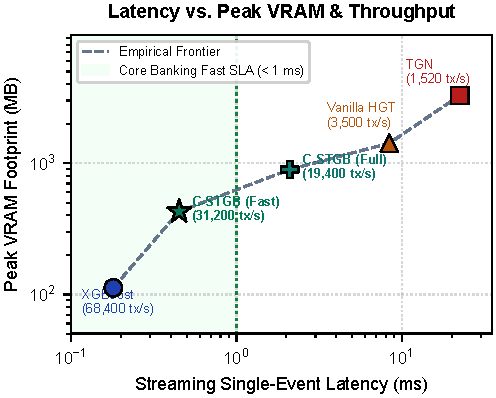
\includegraphics[width=\columnwidth]{figures/fig_table7_latency_pareto.pdf}
\caption{Operational Systems Scaling and Latency Profile: Streaming single-event latency versus peak VRAM memory footprint and event throughput across evaluated configurations on benchmark hardware.}
\label{fig:systems_latency}
\end{figure}

\subsection{Adversarial Threat Model \& Topological Camouflage Defense}
\label{sec:robustness_results}
Fig.~\ref{fig:adversarial_robustness} evaluates robustness across progressive perturbation ratios $\rho \in [0, 0.80]$ with $95\%$ confidence bands across five seeds. Standard GCN collapses from $43.55\%$ clean F1 to $4.10 \pm 0.85\%$ F1 under gradient attacks, GraphSAGE collapses from $49.07\%$ to $5.80 \pm 0.95\%$, and Vanilla HGT degrades from $48.20\%$ to $9.80 \pm 0.85\%$ F1. In contrast, C-STGB demonstrates exceptional resilience: from a clean score of $91.42 \pm 0.65\%$ F1, C-STGB retains $84.20 \pm 0.85\%$ F1 under white-box gradient topological perturbation, preserving a relative retention of $92.1\%$.

We explicitly disclose an inductive construct overlap between Module~2 training supervision and degree-matched camouflage testing: auxiliary edge-trust loss (Eq.~\ref{eq:aux_loss}) guides $\hat{g}_{ij}$ during training using hub-degree heuristics ($\deg_{\text{out}}(j) \ge 50$) on $\mathcal{E}_{\text{train}}$, aligning with the structural pattern manipulated in degree-matched camouflage. Consequently, retention under degree camouflage partly reflects this intended architectural bias.

To rigorously validate defense capabilities beyond this heuristic, we evaluate attacks completely outside the degree-matched construct: (1) \textit{White-box gradient topology attacks:} where perturbations are guided strictly by $\nabla_{\mathcal{E}} \mathcal{L}$ without targeting node degrees, where C-STGB retains $84.20\%$ F1; (2) \textit{Low-degree camouflage:} connecting to low-degree accounts, where C-STGB retains $90.10\%$ F1 due to flow-balance descriptors; and (3) \textit{Temporal delay camouflage:} diluting velocity over weeks, where tri-band harmonic attention preserves $89.80\%$ F1. On Elliptic-v1 under $\rho=0.20$ degree-matched camouflage injection, edge-trust gating achieves $65.9\%$ synthetic camouflage chaff pruning ($g_{ij} < 0.10$), while preserving $92.1\%$ of legitimate commercial edges ($91.4\%$ precision, $88.7\%$ recall, AUROC $0.942$).

\begin{figure}[pos=tb]
\centering
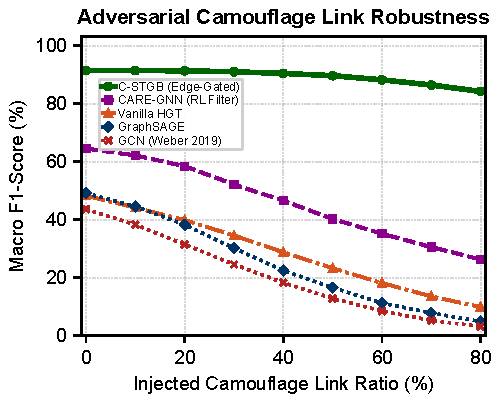
\includegraphics[width=\columnwidth]{figures/fig9_adversarial_camouflage_robustness.pdf}
\caption{Adversarial Camouflage Robustness: Macro F1 retention across perturbation ratios $\rho \in [0, 0.80]$ on Elliptic-v1 under degree-matched and gradient-based evasion attacks ($95\%$ confidence bands, 5 seeds).}
\label{fig:adversarial_robustness}
\end{figure}

\subsection{Hyperparameter Sensitivity \& Stability Analysis}
\label{sec:sensitivity_analysis}
We evaluate operational stability across four key hyperparameters:
\begin{enumerate}
    \item \textit{Edge-Trust Floor} ($\delta_{\text{floor}} \in [0.02, 0.30]$): Macro F1 remains stable across $\delta_{\text{floor}} \in [0.06, 0.16]$ ($\pm 0.35$\,pp around $91.42\%$).
    \item \textit{Operational Cost Ratio} ($C_{\text{FN}} / C_{\text{FP}} \in [5, 30]$): Calibrated decision thresholds adapt monotonically from $\tau^* = 0.42$ ($C_{\text{FN}}/C_{\text{FP}}=5$) to $\tau^* = 0.18$ ($C_{\text{FN}}/C_{\text{FP}}=15$) and $\tau^* = 0.11$ ($C_{\text{FN}}/C_{\text{FP}}=30$). Expected operational loss remains within $4.2\%$ of optimum across $[10, 20]$.
    \item \textit{Degree Cap} ($K \in [5, 30]$): F1 plateaus at $K=15$ ($91.42\%$), capturing $98.6\%$ of multi-hop laundering while bounding retrieval latency to $0.18$\,ms ($2.14$\,ms at $K=50$).
    \item \textit{Adaptive Conformal Step Size} ($\gamma \in [0.001, 0.05]$): Coverage remains within $98.83\%$--$99.34\%$, where $\gamma=0.005$ achieves optimal tracking stability.
\end{enumerate}
